\begin{figure}[htbp]
  \centering
  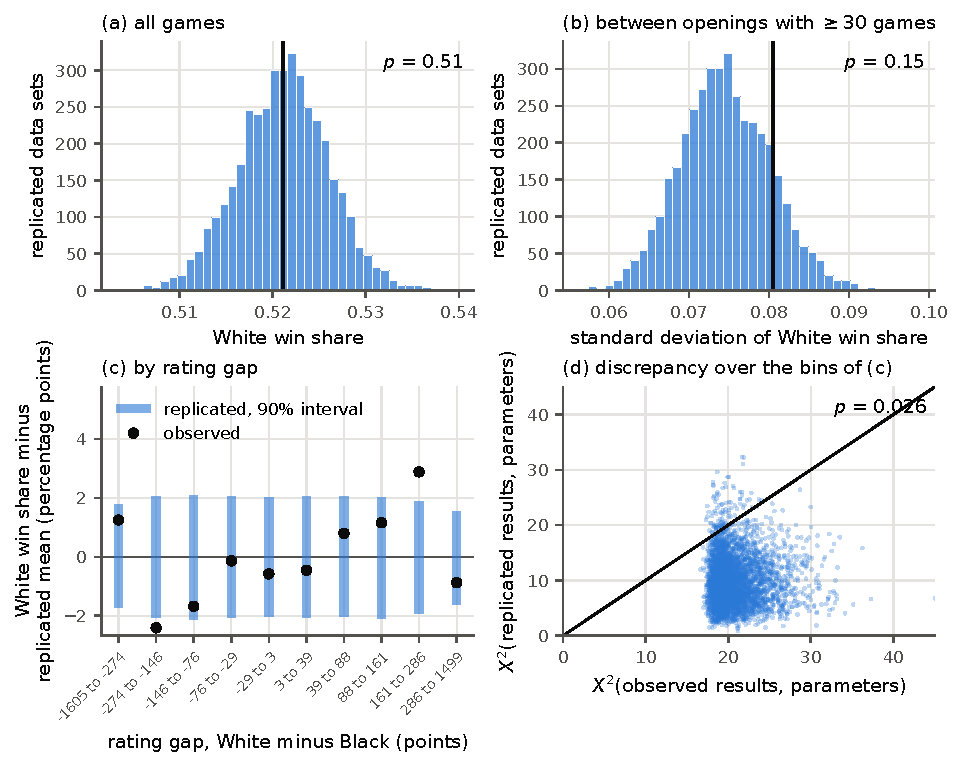
\includegraphics[width=\linewidth]{posterior_predictive.pdf}
  \caption{Posterior predictive checks, from 4,000 data sets simulated from the posterior for the real rating gaps and openings. (a), (b): histograms of the replicated statistic; the black line is the observed value and $p$ the share of replicated values at least as large. (c): observed White win share in each decile of rating gap, minus the mean of its replicated values, with the central 90\% interval of the replicated values. (d): chi-square discrepancy between wins and expected wins over the deciles of (c), for the observed and the replicated results under the same posterior draw; points below the line are draws where the observed results fit worse than the replicated ones. The model reproduces the overall win share ($p = 0.51$) and the spread between openings ($p = 0.15$), but not the shape of the win share against the rating gap ($p = 0.026$): the stronger player wins more often than predicted at moderate gaps, for example 74.1\% observed against 71.2\% replicated for gaps of 161 to 286 points.}
  \label{fig:posterior_predictive}
\end{figure}
